% Options for packages loaded elsewhere
\PassOptionsToPackage{unicode}{hyperref}
\PassOptionsToPackage{hyphens}{url}
\documentclass[
  ignorenonframetext,
]{beamer}
\newif\ifbibliography
\usepackage{pgfpages}
\setbeamertemplate{caption}[numbered]
\setbeamertemplate{caption label separator}{: }
\setbeamercolor{caption name}{fg=normal text.fg}
\beamertemplatenavigationsymbolsempty
% remove section numbering
\setbeamertemplate{part page}{
  \centering
  \begin{beamercolorbox}[sep=16pt,center]{part title}
    \usebeamerfont{part title}\insertpart\par
  \end{beamercolorbox}
}
\setbeamertemplate{section page}{
  \centering
  \begin{beamercolorbox}[sep=12pt,center]{section title}
    \usebeamerfont{section title}\insertsection\par
  \end{beamercolorbox}
}
\setbeamertemplate{subsection page}{
  \centering
  \begin{beamercolorbox}[sep=8pt,center]{subsection title}
    \usebeamerfont{subsection title}\insertsubsection\par
  \end{beamercolorbox}
}
% Prevent slide breaks in the middle of a paragraph
\widowpenalties 1 10000
\raggedbottom
\AtBeginPart{
  \frame{\partpage}
}
\AtBeginSection{
  \ifbibliography
  \else
    \frame{\sectionpage}
  \fi
}
\AtBeginSubsection{
  \frame{\subsectionpage}
}
\usepackage{iftex}
\ifPDFTeX
  \usepackage[T1]{fontenc}
  \usepackage[utf8]{inputenc}
  \usepackage{textcomp} % provide euro and other symbols
\else % if luatex or xetex
  \usepackage{unicode-math} % this also loads fontspec
  \defaultfontfeatures{Scale=MatchLowercase}
  \defaultfontfeatures[\rmfamily]{Ligatures=TeX,Scale=1}
\fi
\usepackage{lmodern}
\ifPDFTeX\else
  % xetex/luatex font selection
\fi
% Use upquote if available, for straight quotes in verbatim environments
\IfFileExists{upquote.sty}{\usepackage{upquote}}{}
\IfFileExists{microtype.sty}{% use microtype if available
  \usepackage[]{microtype}
  \UseMicrotypeSet[protrusion]{basicmath} % disable protrusion for tt fonts
}{}
\makeatletter
\@ifundefined{KOMAClassName}{% if non-KOMA class
  \IfFileExists{parskip.sty}{%
    \usepackage{parskip}
  }{% else
    \setlength{\parindent}{0pt}
    \setlength{\parskip}{6pt plus 2pt minus 1pt}}
}{% if KOMA class
  \KOMAoptions{parskip=half}}
\makeatother
\usepackage{longtable,booktabs,array}
\newcounter{none} % for unnumbered tables
\usepackage{calc} % for calculating minipage widths
\usepackage{caption}
% Make caption package work with longtable
\makeatletter
\def\fnum@table{\tablename~\thetable}
\makeatother
\usepackage{graphicx}
\makeatletter
\newsavebox\pandoc@box
\newcommand*\pandocbounded[1]{% scales image to fit in text height/width
  \sbox\pandoc@box{#1}%
  \Gscale@div\@tempa{\textheight}{\dimexpr\ht\pandoc@box+\dp\pandoc@box\relax}%
  \Gscale@div\@tempb{\linewidth}{\wd\pandoc@box}%
  \ifdim\@tempb\p@<\@tempa\p@\let\@tempa\@tempb\fi% select the smaller of both
  \ifdim\@tempa\p@<\p@\scalebox{\@tempa}{\usebox\pandoc@box}%
  \else\usebox{\pandoc@box}%
  \fi%
}
% Set default figure placement to htbp
\def\fps@figure{htbp}
\makeatother
\setlength{\emergencystretch}{3em} % prevent overfull lines
\providecommand{\tightlist}{%
  \setlength{\itemsep}{0pt}\setlength{\parskip}{0pt}}
% Slide layout defaults for warning-clean scientific decks.
\usepackage{etoolbox}
\IfFileExists{xurl.sty}{\usepackage{xurl}}{}
\IfFileExists{seqsplit.sty}{\usepackage{seqsplit}}{\newcommand{\seqsplit}[1]{#1}}
\protected\def\breakseq#1{\seqsplit{#1}}
\protected\def\breaktt#1{\begingroup\ttfamily\seqsplit{#1}\endgroup}
\setlength{\emergencystretch}{6em}
\tolerance=5000
\hbadness=10000
\hfuzz=1pt
\setlength{\tabcolsep}{2pt}
\AtBeginEnvironment{longtable}{\tiny\renewcommand{\arraystretch}{0.86}\setlength{\tabcolsep}{1pt}}
\AtBeginEnvironment{tabular}{\tiny\renewcommand{\arraystretch}{0.86}\setlength{\tabcolsep}{1pt}}

% Natbib and cross-reference fallbacks — slides don't load natbib
% or cleveref, but combined-PDF manuscript prose may emit these
% commands. The fallback renders citations as a bracketed key list
% and cross-references as detokenized labels so slides don't fail on
% undefined control sequences or raw underscores. \providecommand is
% a no-op if packages load later.
\providecommand{\citep}[1]{[#1]}
\providecommand{\citet}[1]{#1}
\providecommand{\citealp}[1]{#1}
\providecommand{\citeauthor}[1]{#1}
\providecommand{\citeyear}[1]{#1}
\providecommand{\cref}[1]{\texttt{\detokenize{#1}}}
\providecommand{\Cref}[1]{\texttt{\detokenize{#1}}}

\newtheorem{proposition}{Proposition}
\newtheorem{hypothesis}{Hypothesis}
\usepackage{bookmark}
\IfFileExists{xurl.sty}{\usepackage{xurl}}{} % add URL line breaks if available
\urlstyle{same}
% fallback for those not using the hyperref driver hyperxmp:
\makeatletter
\@ifundefined{xmpquote}{\newcommand{\xmpquote}[1]{#1}}{}
\makeatother
\hypersetup{
  hidelinks,
  pdfcreator={LaTeX via pandoc}}

\author{\texorpdfstring{}{}}
\date{}

\begin{document}

\section{Results: Hypotheses
Explored}\label{results-hypotheses-explored}

\begin{frame}[allowframebreaks]{Results: Hypotheses Explored}
The template scores a configurable set of hypotheses about the topic.
For this instance 6 hypotheses are declared in configuration; Table 7
lists them with their scope and evidence score.

\textbf{Table 7. Hypotheses explored.}

{\def\LTcaptype{none} % do not increment counter
\begin{longtable}[]{@{}llll@{}}
\toprule\noalign{}
ID & Hypothesis & Scope & Evidence score \\
\midrule\noalign{}
\endhead
H1 & Wakefulness Efficacy & clinical & +0.00 \\
H2 & Cognitive Enhancement & cognitive & +0.00 \\
H3 & Low Abuse Liability & safety & +0.00 \\
H4 & Dopaminergic Mechanism & pharmacological & +0.00 \\
H5 & Off-label Psychiatric Utility & applied & +0.00 \\
H6 & Tolerability & safety & +0.00 \\
\bottomrule\noalign{}
\end{longtable}
}

Evidence scores are produced by the optional, LLM-gated knowledge-graph
stage. In the offline default run that stage does not execute, so scores
read \emph{pending} --- the hypotheses, their names, and their scope are
nonetheless reported directly from configuration. A live run with a
language model available populates the scores from citation-weighted
assertion extraction.
\end{frame}

\begin{frame}[allowframebreaks]{Interpretation}
\protect\phantomsection\label{interpretation}
Reported scores, when present, should be read as relative rankings
rather than calibrated probabilities: absolute magnitudes are inflated
by publication bias and the linguistic asymmetry of academic writing. A
positive score indicates that the retrieved corpus \emph{talks about}
the hypothesis in a supporting direction; a negative score indicates
contradicting evidence; a score near zero indicates either balanced
evidence or insufficient coverage.

The six hypotheses frame the evidence landscape for Modafinil:

\begin{itemize}
\item
  \textbf{H1 (Wakefulness Efficacy)} --- the clinical claim that
  modafinil reliably promotes wakefulness in sleep-disorder populations.
  This is the primary indication and the most-studied claim in the
  corpus.
\item
  \textbf{H2 (Cognitive Enhancement)} --- the claim that modafinil
  improves attention, working memory, and executive function, especially
  under sleep deprivation. This hypothesis drives the neuroenhancement
  literature and is the subject of significant public and scientific
  debate.
\item
  \textbf{H3 (Low Abuse Liability)} --- the safety claim that modafinil
  has lower abuse potential than classical psychostimulants. This is
  critical for regulatory classification and prescribing decisions.
\item
  \textbf{H4 (Dopaminergic Mechanism)} --- the pharmacological claim
  that modafinil acts substantially via dopamine-transporter inhibition
  rather than a purely novel mechanism. This hypothesis has mechanistic
  and translational implications.
\item
  \textbf{H5 (Off-label Psychiatric Utility)} --- the applied claim that
  modafinil is a useful adjunct for fatigue and cognition in psychiatric
  and neurological conditions, including depression, ADHD, and
  schizophrenia.
\item
  \textbf{H6 (Tolerability)} --- the safety claim that modafinil is
  generally well tolerated, with predominantly mild, transient adverse
  effects. This underpins its clinical acceptability relative to
  alternative wakefulness agents.
\end{itemize}

\pandocbounded{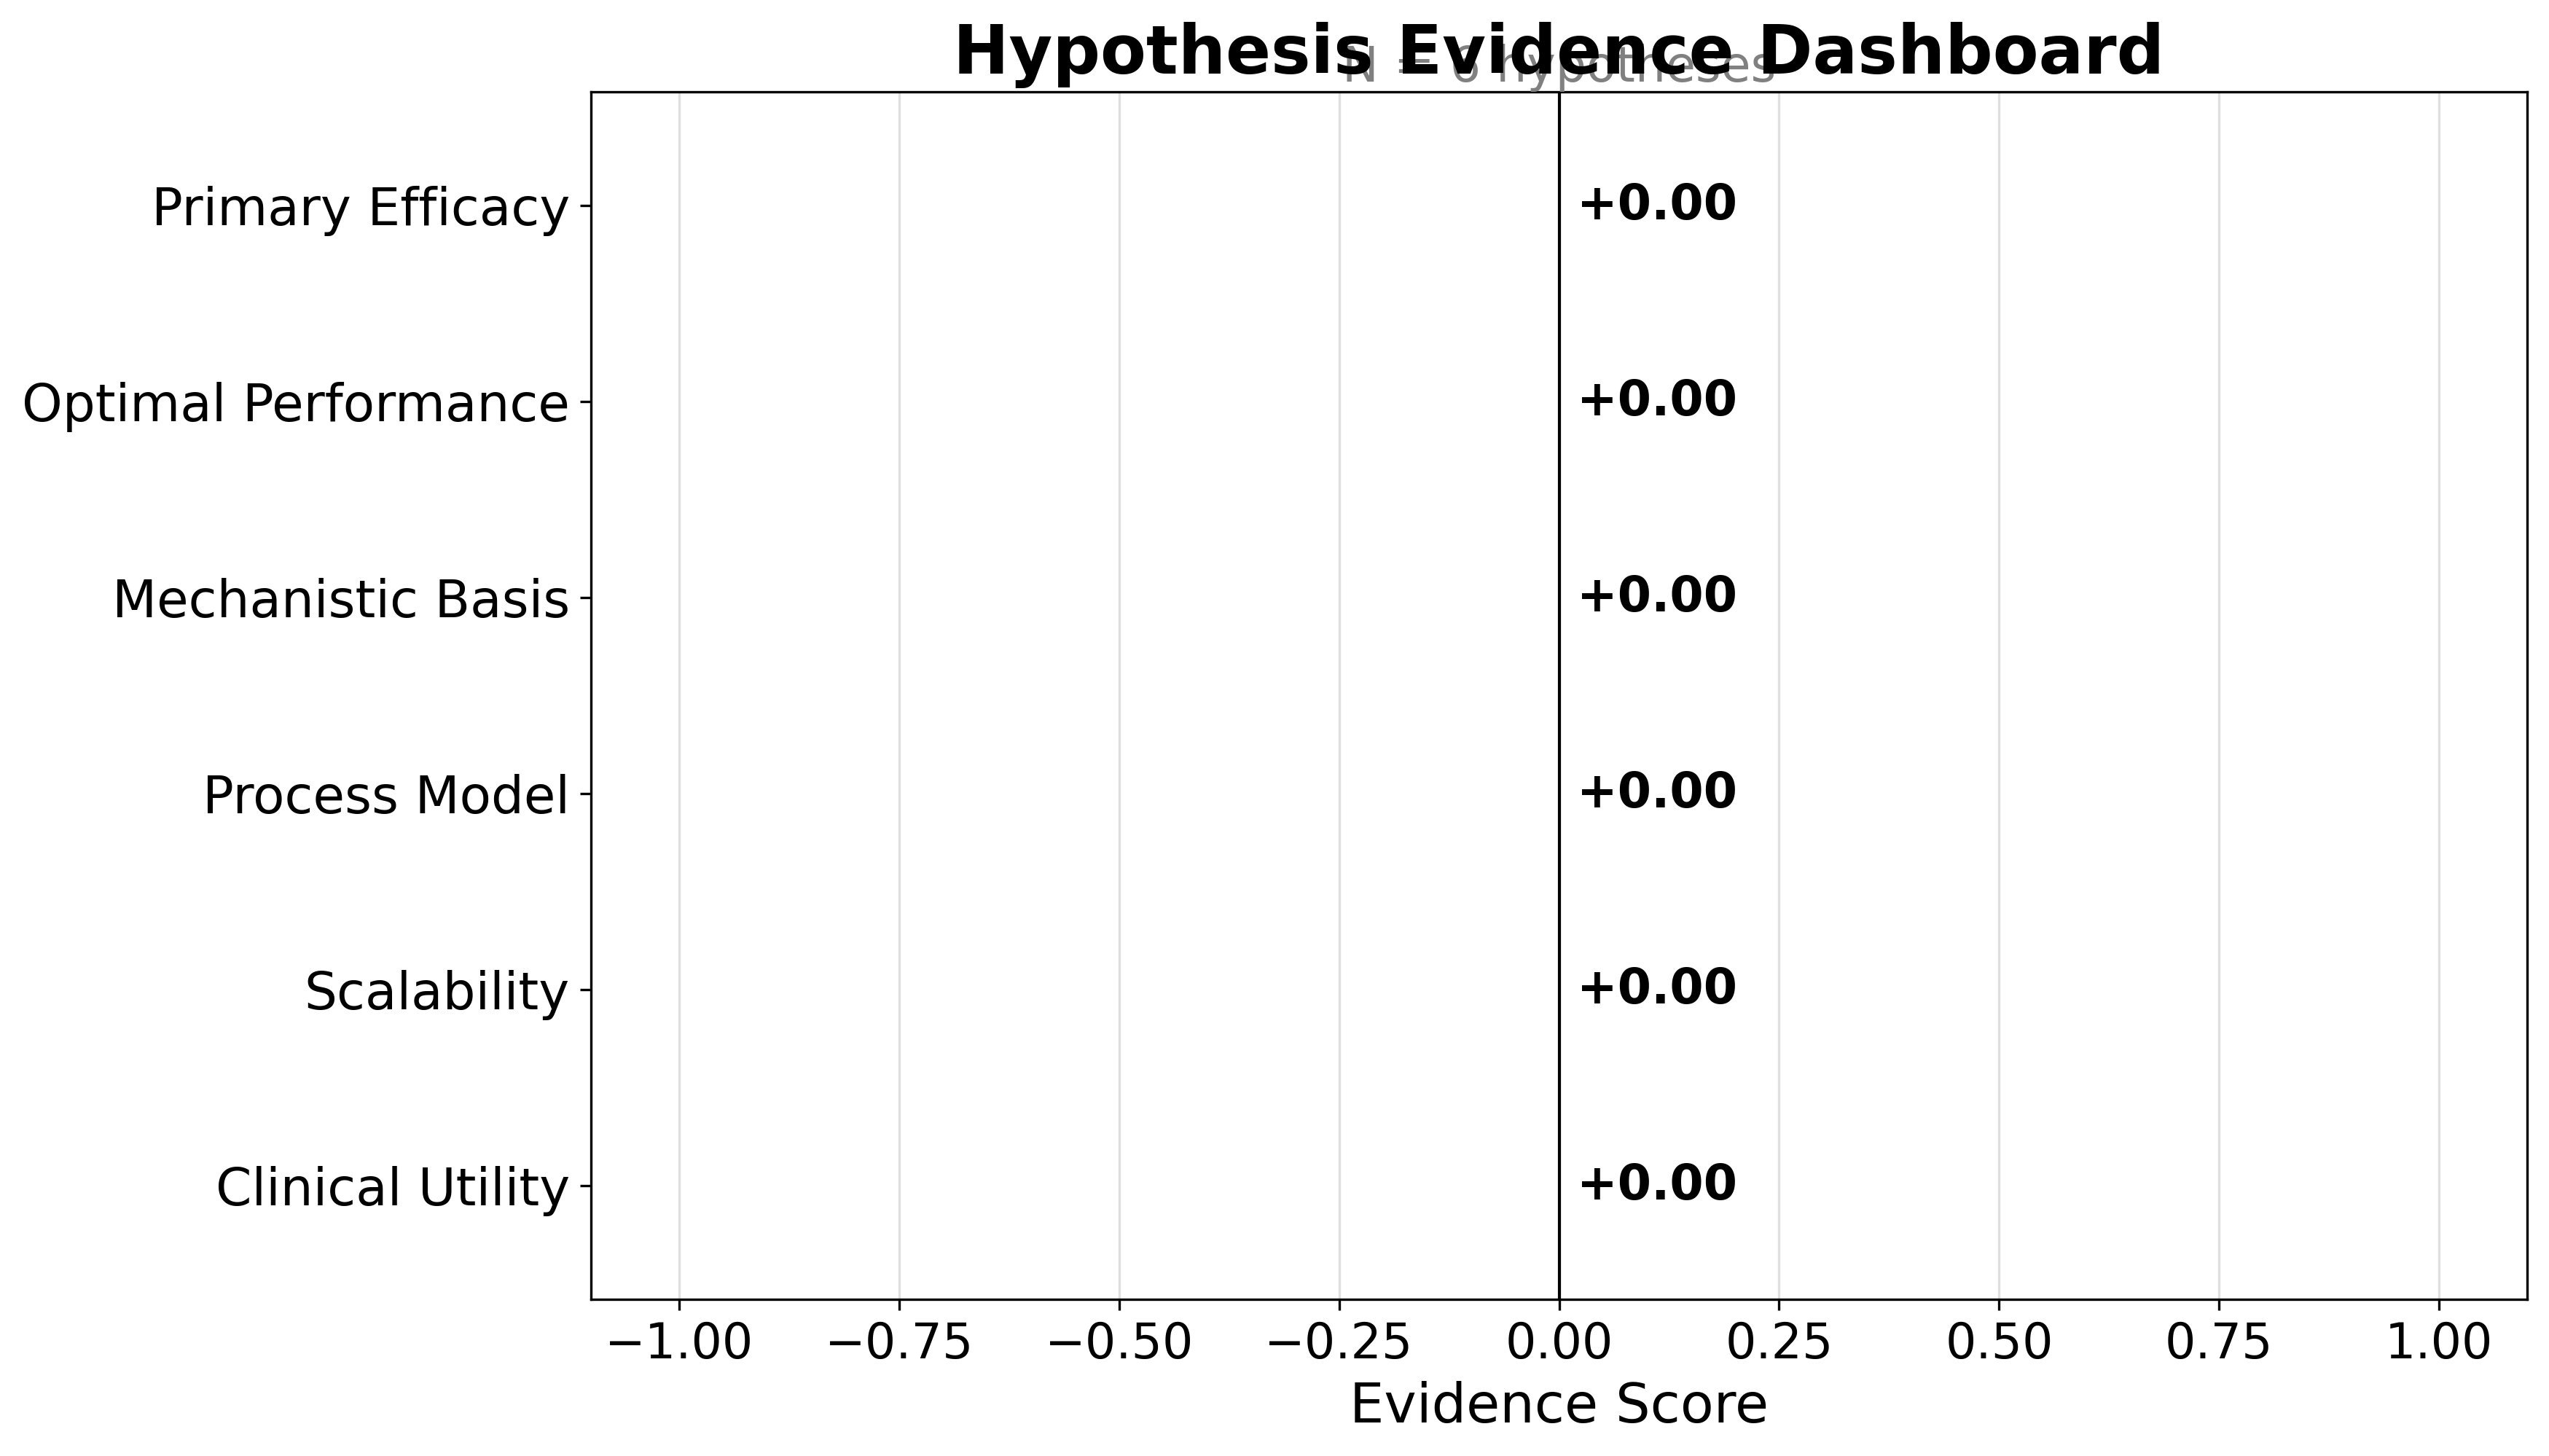
\includegraphics[keepaspectratio,alt={Hypothesis dashboard for Modafinil. The dashboard summarizes the evidence scores across the 6 configured hypotheses, showing the direction and magnitude of citation-weighted assertion evidence.}]{../figures/hypothesis_dashboard.png}}\{\{\#fig:hypothesis\_dashboard\}\}
\end{frame}

\end{document}
